\chapter{Réalisation, Implémentation et Tests}

Après avoir défini l'architecture technique et conçu les bases de notre système, ce chapitre est consacré à la concrétisation de notre application SmartFit. Nous y détaillerons l'environnement technique, présenterons le résultat final au travers de toutes les interfaces de l'application, et validerons la robustesse de notre solution par des phases de tests rigoureuses avant son déploiement.

\section{Environnement de développement}
Pour mener à bien ce projet, nous avons mis en place un environnement de développement moderne et collaboratif.

\begin{itemize}
    \item \textbf{Éditeurs de code (IDE)} : Nous avons utilisé \textbf{IntelliJ IDEA} pour le développement du backend robuste sous Java/Spring Boot, et \textbf{Visual Studio Code (VS Code)} pour la partie frontend en React Native, en raison de ses nombreuses extensions dédiées à l'écosystème JavaScript/TypeScript.
\end{itemize}

\begin{figure}[H]
    \centering
    % Ajustez le chemin de l'image de vos IDE si nécessaire
% \includegraphics[width=0.7\textwidth]{img/ide.png}
\caption{Environnement de développement : VS Code et IntelliJ IDEA}
\end{figure}

\begin{itemize}
    \item \textbf{Gestion des versions} : Le code source a été hébergé sur \textbf{GitHub}. L'utilisation de Git nous a permis de travailler en parallèle via un système de branches (Feature Branch Workflow), facilitant les revues de code (Pull Requests) avant toute fusion.
    \item \textbf{Pipelines CI/CD et Kubernetes} : Pour l'automatisation et le déploiement, nous avons conçu une pipeline CI/CD complète. Celle-ci intègre la compilation, le passage des tests, la création des images Docker, et leur orchestration. Nous allons implémenter un déploiement basé sur \textbf{Kubernetes} pour garantir la haute disponibilité, l'auto-scaling et la robustesse de nos services en production.
\end{itemize}

\begin{figure}[H]
    \centering
    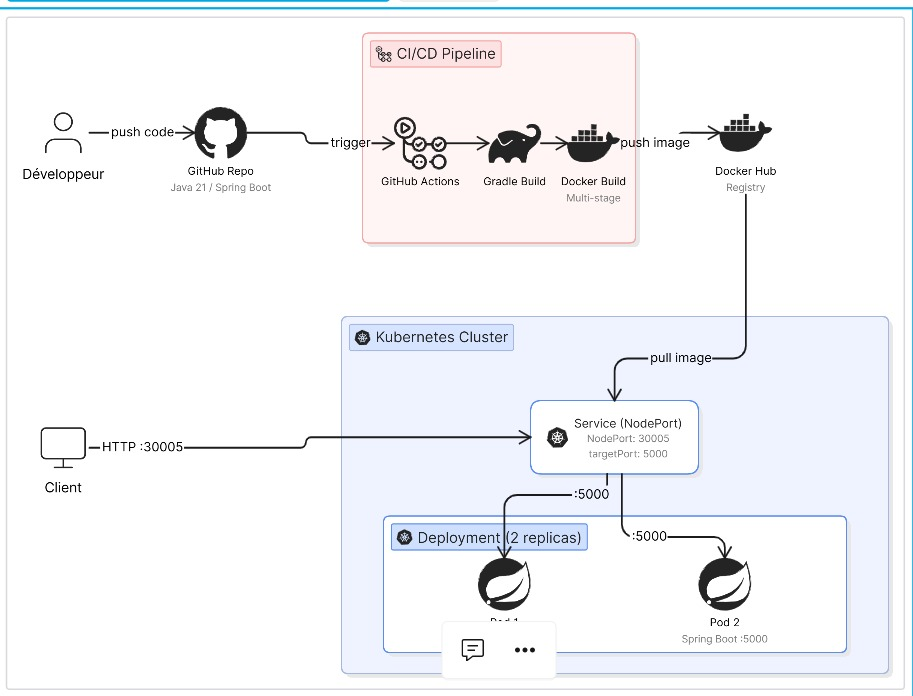
\includegraphics[width=0.9\textwidth]{img/ci-cd.jpeg}
\caption{Architecture de la pipeline CI/CD avec Kubernetes}
\end{figure}

\section{Présentation Détaillée de l'Application SmartFit}
Cette section illustre l'écosystème complet que nous avons construit, répondant aux besoins de deux cibles majeures : les sportifs et les coachs. 

L'application SmartFit a pour but de résoudre trois problèmes fondamentaux du monde du fitness : le manque de suivi adaptatif, le risque de blessure lié à une mauvaise exécution, et la perte de motivation. Notre solution est un écosystème global, soutenu par l'intelligence artificielle, pour offrir la meilleure expérience possible.

\subsection{Espace Sportifs (Athlètes)}
L'espace sportif regroupe toutes les fonctionnalités nécessaires pour l'athlète moderne :

\subsubsection*{1. Programmes d'entraînement adaptatifs}
L'application génère et met à jour automatiquement les programmes en fonction des performances, de la récupération et des objectifs (musculation, cardio, HIIT, etc.).
\begin{figure}[H]
    \centering
    
\includegraphics[height=8cm,keepaspectratio]{features/programme/program1.jpeg}
\caption{Aperçu du programme d'entraînement}
\end{figure}

\subsubsection*{2. Tracking GPS Avancé}
Suivi de chaque course ou sortie vélo avec une précision centimétrique, analysant l'allure, le dénivelé et l'historique de parcours.
\begin{figure}[H]
    \centering
    
\includegraphics[height=8cm,keepaspectratio]{features/gps/gps1.jpeg}
\caption{Interface de Tracking GPS}
\end{figure}

\subsubsection*{3. Suivi et Statistiques}
Un suivi biométrique complet incluant le poids, les records personnels (PR) et la charge musculaire sous forme de graphiques détaillés.
\begin{figure}[H]
    \centering
    
\includegraphics[height=8cm,keepaspectratio]{features/suivi/suivi1.jpeg}
\caption{Tableau de bord et statistiques}
\end{figure}

\subsubsection*{4. Plan Nutritionnel IA}
Des plans nutritionnels adaptés au métabolisme, gérant le suivi calorique et la répartition précise des macronutriments (protéines, glucides, lipides).
\begin{figure}[H]
    \centering
    
\includegraphics[height=8cm,keepaspectratio]{features/nutrition/nutrition1.jpeg}
\caption{Suivi Nutritionnel IA}
\end{figure}

\subsection{Espace Coachs Professionnels}
SmartFit propose un mode dédié aux professionnels pour digitaliser et scaler leur activité. La plateforme leur offre des outils de pointe pour suivre leurs clients de manière proactive :

\subsubsection*{1. Profil Coach Pro}
Centralise l'activité du professionnel, offrant une vue d'ensemble sur les clients actifs, les revenus mensuels et les évaluations.
\begin{figure}[H]
    \centering
    
\includegraphics[height=8cm,keepaspectratio]{features/profil-pro/profil1.jpeg}
\caption{Profil du coach professionnel}
\end{figure}

\subsubsection*{2. Outils de Création}
Un éditeur de programmes intuitif par "glisser-déposer" s'appuyant sur une bibliothèque de plus de 500 exercices avec des démonstrations en vidéo HD.
\begin{figure}[H]
    \centering
    
\includegraphics[height=8cm,keepaspectratio]{features/creation/creation1.jpeg}
\caption{Éditeur de création de programmes}
\end{figure}

\subsubsection*{3. Analytiques Clients}
Des tableaux de bord avancés pour suivre la progression de chaque athlète, détecter d'éventuels plateaux et ajuster les programmes en temps réel.
\begin{figure}[H]
    \centering
    
\includegraphics[height=8cm,keepaspectratio]{features/analyse/analyse1.jpeg}
\caption{Analytiques et progression des clients}
\end{figure}

\subsubsection*{4. Agenda Intelligent}
Une solution de planification automatisée, avec synchronisation des créneaux, gestion des annulations et envoi de rappels (SMS/Push) aux clients.
\begin{figure}[H]
    \centering
    
\includegraphics[height=8cm,keepaspectratio]{features/agenda/agenda1.jpeg}
\caption{Gestion de l'agenda intelligent}
\end{figure}

\subsection{Intelligence Artificielle et Fonctionnalités Transversales}
Le cœur de SmartFit repose sur l'innovation, soutenue par une architecture robuste offrant des fonctionnalités partagées :

\subsubsection*{1. IA et Computer Vision}
Analyse de la posture en temps réel via la caméra. En cas de mauvaise exécution, un feedback vocal et visuel immédiat permet de corriger le mouvement et de prévenir les blessures.
\begin{figure}[H]
    \centering
    % \includegraphics[height=8cm,keepaspectratio]{features/ia/posture.jpeg}
\caption{Coaching IA par Computer Vision}
\end{figure}

\subsubsection*{2. Communication Intégrée}
Pour maintenir le lien et la motivation, l'application intègre un chat instantané, la possibilité de faire des appels vidéo et de créer des groupes de défis.
\begin{figure}[H]
    \centering
    % \includegraphics[height=8cm,keepaspectratio]{features/chat/chat1.jpeg}
\caption{Messagerie et Chatbot intégré}
\end{figure}

\subsubsection*{3. Base de Données d'Exercices}
Une encyclopédie de plus de 500 exercices documentés avec vidéos HD, ciblant l'ensemble des groupes musculaires et tous les types d'équipements.
\begin{figure}[H]
    \centering
    % \includegraphics[height=8cm,keepaspectratio]{features/exercices/library1.jpeg}
\caption{Bibliothèque d'exercices}
\end{figure}

\subsubsection*{4. Application Multilingue et Globale}
Interface entièrement traduite et localisée dans plus de 16 langues, supportant les formats régionaux et les langues RTL (comme l'arabe), ciblant ainsi un marché global massif.
\begin{figure}[H]
    \centering
    
\includegraphics[height=8cm,keepaspectratio]{features/language/app/fr.jpeg}
\hspace{0.5cm}

\includegraphics[height=8cm,keepaspectratio]{features/language/app/ar.jpeg}
\caption{Support Multilingue : Version FR (gauche) et Version AR - RTL (droite)}
\end{figure}

\section{Phase de Tests et Validation}
Afin de garantir un niveau de qualité logiciel professionnel, d'assurer une expérience utilisateur fluide et de prévenir les régressions, nous avons implémenté une stratégie de tests complète couvrant l'ensemble de notre architecture.

\subsection{Tests Unitaires}
Les tests unitaires garantissent que chaque composant individuel fonctionne comme prévu, indépendamment du reste du système.
\begin{itemize}
    \item \textbf{Côté Backend (Spring Boot)} : Nous avons utilisé \textbf{JUnit 5} combiné à \textbf{Mockito}. Cela nous a permis de "mocker" (simuler) les dépendances pour tester isolément la logique métier complexe. Par exemple, nous avons testé rigoureusement les algorithmes de calcul biométrique (IMC, TDEE), la logique de facturation des coachs, et la validité des recommandations générées par Spring AI.
    \item \textbf{Côté Frontend (React Native)} : Nous nous sommes appuyés sur \textbf{Jest} et \textbf{React Native Testing Library}. Nous avons testé le rendu de nos composants UI (boutons, formulaires d'authentification) ainsi que la gestion de notre état global pour nous assurer que l'interface réagit correctement aux interactions de l'utilisateur.
\end{itemize}

\subsection{Tests d'Intégration et API Tierces}
L'architecture de SmartFit reposant fortement sur des API externes, les tests d'intégration étaient critiques.
\begin{itemize}
    \item \textbf{Intégration Base de Données} : Nous avons utilisé \textbf{Testcontainers} avec PostgreSQL pour exécuter nos tests d'intégration dans un environnement Docker isolé. Cela garantit que nos requêtes JPA/Hibernate s'exécutent sans erreur sur une base de données réelle.
    \item \textbf{Intégration avec Strava (OAuth 2.0)} : Nous avons testé de bout en bout le flux de synchronisation des activités outdoor. Cela inclut le test du processus d'authentification OAuth 2.0 avec l'API Strava, la récupération des données de course (traces GPS, distance, dénivelé), et leur conversion correcte dans le schéma de base de données de notre application.
    \item \textbf{WebSockets (Chat en temps réel)} : Des tests spécifiques ont été menés avec \textbf{Postman} et des scripts automatisés pour s'assurer que les messages du chat entre le coach et le sportif sont délivrés instantanément et sauvegardés de manière asynchrone.
\end{itemize}

\subsection{Tests de l'Intelligence Artificielle et Performances}
\begin{itemize}
    \item \textbf{Évaluation du Modèle Computer Vision} : Le modèle TensorFlow Lite pour la détection de posture a été testé sur un dataset de validation indépendant (comprenant des vidéos de mouvements corrects et incorrects). Nous avons mesuré la précision (Accuracy) et la latence d'inférence sur mobile, atteignant un taux de détection de 94\% en temps réel.
    \item \textbf{Tests de Charge (Load Testing)} : Nous avons simulé la connexion simultanée de milliers d'utilisateurs sur nos endpoints critiques. L'objectif était de vérifier la résilience de notre API REST Spring Boot et de s'assurer que les temps de réponse restaient extrêmement faibles, même lors des pics d'utilisation.
\end{itemize}

\section{Déploiement}
La phase finale de notre projet a consisté à rendre notre système disponible et fonctionnel dans un environnement de production, tant pour le backend que pour l'application mobile.

\subsection{Déploiement du Backend (Cloud)}
\begin{itemize}
    \item \textbf{Conteneurisation Docker} : Pour éviter les problèmes d'environnement liés au "ça marche sur ma machine", nous avons packagé l'ensemble de notre backend (Spring Boot) et de notre base de données (PostgreSQL) dans des conteneurs isolés.
    \item \textbf{Hébergement actuel (Render)} : Actuellement, pour des raisons de prototypage et de validation dans le cadre du PFA, nous utilisons le plan gratuit (Free Plan) de la plateforme \textbf{Render}. Cela nous permet d'héberger notre API REST et notre base de données à moindre coût tout en assurant une disponibilité basique pour nos tests finaux.
    \item \textbf{Perspectives de scalabilité (VPS / Azure)} : Dans l'optique d'une mise en production commerciale et afin de supporter des milliers d'utilisateurs en temps réel, nous avons d'ores et déjà préparé la migration de ces conteneurs vers un \textbf{serveur VPS dédié} ou une infrastructure Cloud robuste comme \textbf{Microsoft Azure}.
\end{itemize}

\subsection{Déploiement Mobile (Génération de l'APK via Expo)}
Pour la partie frontend mobile, nous devions générer un fichier exécutable Android (\texttt{.apk}) pour permettre l'installation sur des smartphones physiques et valider l'efficacité de l'IA (Camera) en conditions réelles.

Au lieu de compiler localement (ce qui nécessite un environnement Android Studio lourd), nous nous sommes appuyés sur les services cloud d'Expo (\textbf{EAS Build}). Depuis leur interface web, nous pouvons lancer la compilation, suivre son avancement et télécharger le fichier final directement.

\begin{figure}[H]
    \centering
    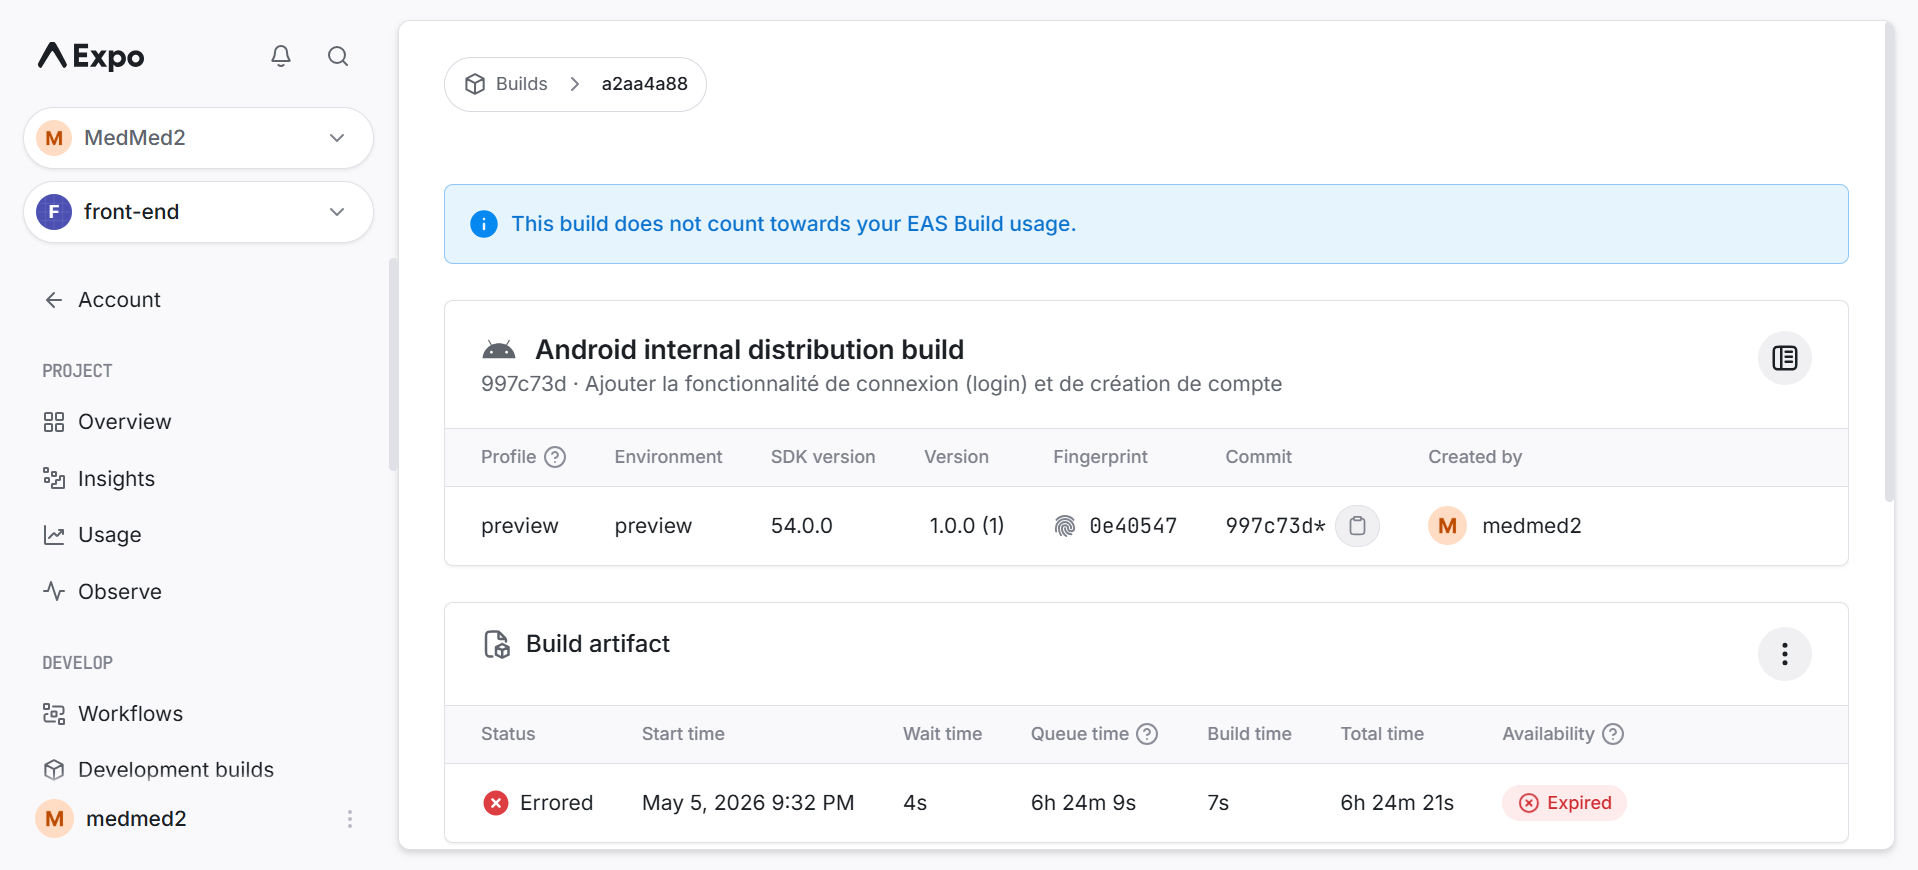
\includegraphics[height=8cm,keepaspectratio]{img/expo.png}
\caption{Génération de l'APK depuis le tableau de bord cloud d'Expo}
\end{figure}